\section{Schwierigkeiten von Vektoruhren}
\subsection{Effizienten Speicherung der Vektoruhren}
% Paper: Concerning the size of clocks 
%        Plausible Clocks Constant Size Logical Clocks for Distributed Systems
Vektor Uhren sind eine relativ einfache und effektive Lösung kausale Ordnung in einem verteilten System herzustellen.
Ihre Definition beherbergt jedoch ihren größten Nachteil.
Die Größe einer Uhr ist nicht konstant.
Für ein verteiltes System mit $n$ Prozessen benötigt eine Vektor Uhr $n$ Komponenten i.d.R. Integer-Zahlen.
Die Folge ist, dass für ein großes verteiltes System alle Vektor Uhren einen entsprechend hohen Speicherbedarf haben.
Dies wirkt sich zum einen negativ auf den Speicherverbrauch der einzelnen Prozesse aus, da je nach Implementierung mehrere Uhren gespeichert werden müssen.
Außerdem fügen die großen Vektor Uhren einen Overhead zu den Nachrichten hinzu und belasten somit den Übertragungsweg.
Offensichtlich ist die Länge der Vektor Uhr direkt proportional zur Anzahl der Prozesse.
Somit skalieren Vektor Uhren schlecht \cite{torres1999plausible}.

Charron-Bost \cite{charron1990concerning} hat bewiesen, dass es innerhalb eines Systems bestehend aus $n$ Nodes immer eine mögliche Kombination an Ereignissen geben kann, bei der die Kausalität ausschließlich mit Vektor Uhren der Länge $n$ erfasst werden kann.
Von daher müssen für alle theoretisch vorkommenden Prozesse innerhalb des Systems eine Komponente in der Uhr reserviert werden.
Dies beinhaltet alle aktuellen Prozesse und auch zukünftige Prozesse die möglicherweise ausgeführt werden könnten.
Es ist natürlich schwer im voraus zu entscheiden wie viele Prozesse potentiell ausgeführt werden und ist daher im Allgemeinen nur bei statischen Systemen gegeben, bei denen also  bei denen also die Anzahl der Prozesse konstant ist.
Daher muss theoretisch eine Vektor Uhr mit einer statischen Länge von $n$ verwendet werden.
Im Folgenden werden verschiedene Verfahren vorgestellt um die Länge von Vektor Uhren zu reduzieren.

Ein pragmatisches Vorgehen um die Länge einer Vektor Uhr in einer annehmbarer Größe zu halten wurde von Amazon in ihrer Dynamo Datenbank \cite{decandia2007dynamo} verfolgt.
Hierbei wird die Länge durch folgendes Kürzungsschema reduziert:
Zu jeder Komponente in der Vektor Uhr wird neben dem Zähler noch die Prozess ID und ein Zeitstempel gehalten.
Der Zeitstempel gibt den Zeitpunkt an, zudem der entsprechende Prozess zuletzt den Datensatz aktualisierte.
Erreicht die Länge der Vektor Uhr einen bestimmten Schwellwert, werden die Komponenten mit den ältesten Zeitstempel aus der Uhr entfernt.
Dieses Verwerfen von Daten kann dazu führen, dass in gewissen Situationen die Kausalität nicht mehr komplett hergestellt werden kann.
Nach eigenen Angaben von \etal{DeCandia} \cite{decandia2007dynamo} trat dieses Problem im Produktiveinsatz jedoch nicht auf und wurde daher nicht weiter analysiert.

\etal{Singhal} \cite{singhal1992efficient} stellten ein einfaches Verfahren vor um den Overhead bei der Nachrichtenübertragung im Durchschnitt zu verringern.
Ihre Technik basiert auf der empirischen Beobachtung, dass nur wenige Prozesse häufig miteinander kommunizieren.
Außerdem ist es wahrscheinlich, dass zwischen zwei aufeinanderfolgend Sende-Ereignisse von Prozess $P_i$ zu $P_j$ nur wenige Komponenten der Vektor Uhr sich ändern.
In diesem Fall ist es unnötig die komplette Uhr mit jeder ausgehenden Nachricht von $P_i$ zu $P_j$ zu übertragen.
Es ist ausreichend nur die Komponenten zu übertragen die sich geändert haben.
Konkret kann bei einer gegeben Uhr $VC$ für jede geänderte Komponenten ein Tupel aus $(a, VC[a])$ übertragen werden, wobei $a$ dem Index des Prozess innerhalb der Uhr entspricht.
Werden Vektor Uhren nach dieser Technik übertragen kann die zu übertragene Datenmenge reduziert werden.
Dabei wird jedoch der lokale Speicherbedarf eines Prozesses erhöht, da dieser zusätzlich speichern muss welche Werte zuletzt zu welchen Prozess geschickt wurden.
Anhand den gespeicherten Vektoren kann er die entsprechenden Tupel auswählen, die an eine Nachricht mit angehängt werden müssen.

\begin{figure}[ht]
    \centering
    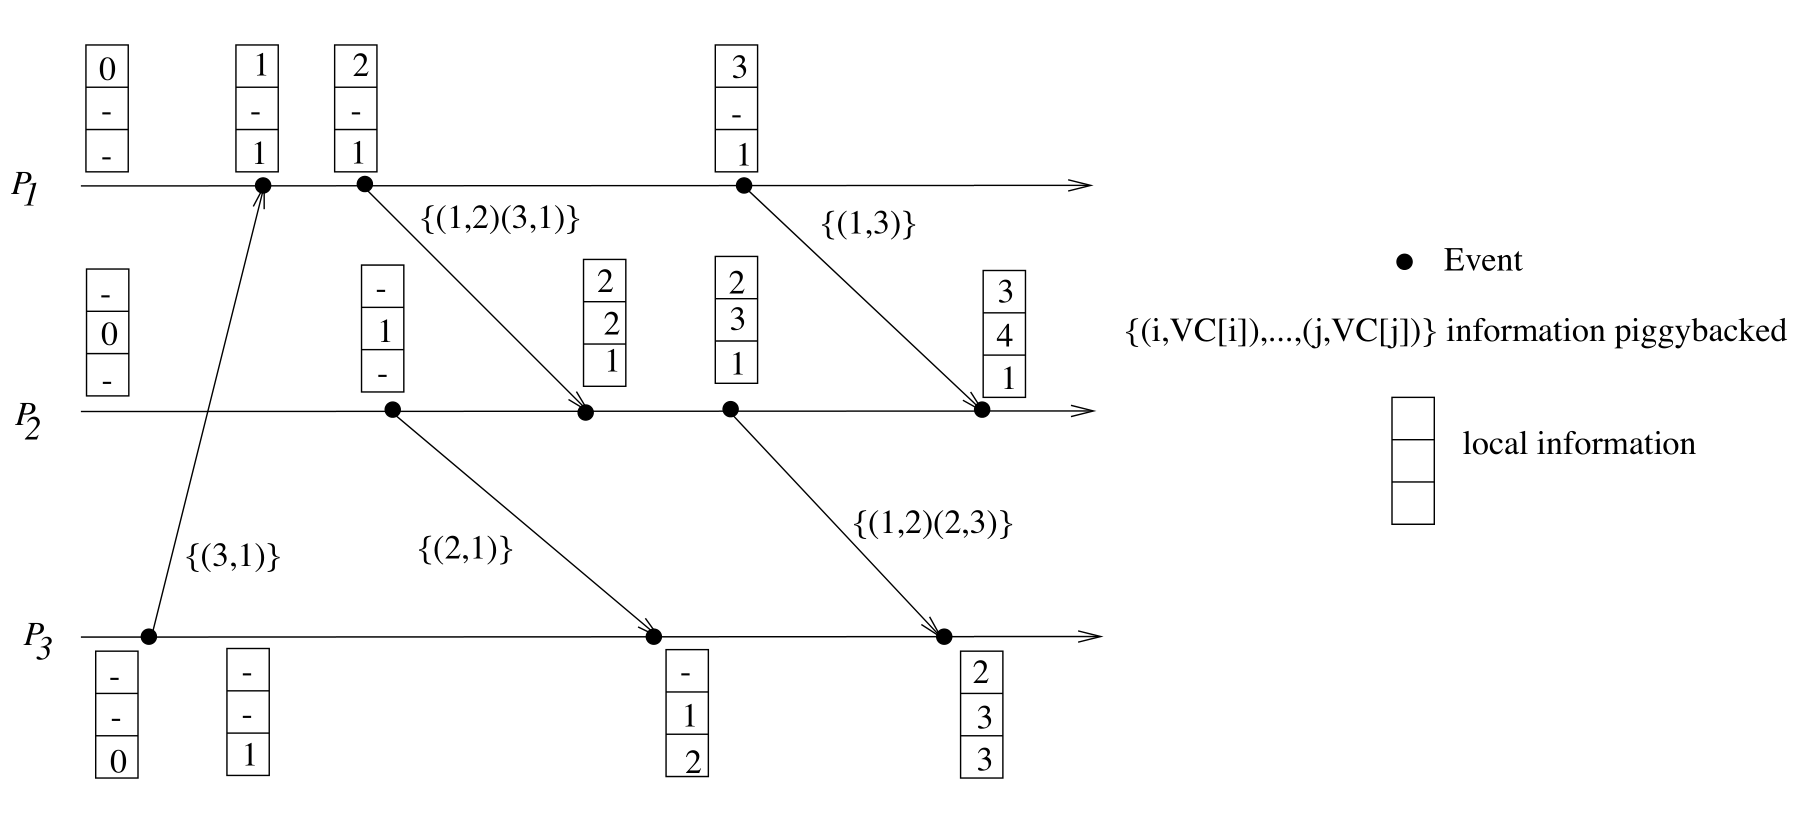
\includegraphics[width=1\textwidth]{Singhal.png}
    \caption[Kommunikaiton nach Singhal]{Ablauf der Kommunikation dreier Prozesse nach dem Verfahren von \etal{Singhal}.}
    Quelle: Nachgezeichnet aus \cite{Baldoni:2002:FDC:1435723.1437765}
    \label{fig:singhal}
\end{figure}

Bisher wurde immer angenommen, dass die Anzahl der Prozesse innerhalb eines Systems konstant ist.
Dies ist jedoch selten der Fall, in der Regel werden Prozesse häufig gestartet und beendet.
Die Folge ist, dass bei einer naiven Implementierung der Vektor Uhr für jeden jemals ausgeführten Prozess eine Komponente in der Uhr reserviert werden muss.
In dynamischen Systemen kann dies dazu führen, dass die Uhren schnell eine tragbare Größe überschreiten.
Es ist daher wünschenswert Vektor Uhren für solche dynamische Systeme zu optimieren.

Fridge \cite{fidge1991logical} stellte ein Modell vor bei dem eine variable Anzahl an Prozess-IDs verwendet wird.
Hierbei müssen die Prozess-IDs innerhalb des Systems eindeutig sein.
Beim Start eines Prozesses wird ihm eine ID zugewiesen.
Die ID eines terminierten Prozesses wird jedoch nicht freigegeben.
Damit die IDs solcher Prozesse freigegeben werden können, müssen allen anderen Prozesse die Terminierung bekannt sein.
Ist dies nicht gegeben, darf die ID nicht aus der Vektor Uhr entfernt werden.
Diese Art von Garbage Collection wird in \cite{richard1998efficient} verwendet.
Alle Verfahren dieser Art haben jedoch das Problem, dass IDs von terminierten Prozessen nicht wiederverwendet werden können und die Bereinigung der Uhr von terminierten Prozessen durch einen einzigen unerreichbaren Prozess bereits verhindert werden kann \cite{almeida2008treeclocks}.

% Hier würde Landes reinpassen

Wie gezeigt führt die Verwendung von globalen IDs zu neuen Problemen.
Es liegt somit nahe auf globale IDs gänzlich zu verzichten.
Aus dieser Überlegung heraus entwickelten \etal{Almeida} \cite{almeida2008treeclocks} eine Generalisierung von Vektor Uhren.
Die sogenannten \qq{Interval Tree Clocks} sind für dynamische Systeme ausgelegt und kommen dabei ohne globale IDs aus, indem jeder Prozess selbständig neue IDs erzeugen, löschen oder wiederverwenden kann, ohne das dabei auf eine globale Kommunikation zurückgegriffen werden muss.
Durch teilen und zusammenfassen von Prozess IDs wachsen und schrumpfen die Zeitstempel entsprechend zu der Dynamik des Systems.
Der Platzbedarf der Zeitstempel skaliert somit mit der Anzahl der Prozesse und wächst nur moderat an \cite{almeida2008treeclocks}.

% \cite{almeida2008treeclocks}
% landes dynamic clock

Ein in der Praxis relevantes Problem ist die Handhabung von Integer Überlaufen der Zählern innerhalb der Uhr.
In der Theorie werden die natürlichen Zahlen als Menge der möglichen Zählerwerte angenommen und haben somit keine Beschränkung.
Bei der Implementierung einer Vektor Uhr muss jedoch über die Darstellung der Vektorkomponenten entschieden werden.
In der Regel wird ein Integer Datentyp mit typischerweise 32 oder 64 Bit gewählt.
Dabei muss ein Kompromiss zwischen maximale Länge und Datenmenge die zu übertragen ist gefunden werden.
Wird das verteilte System lange genug ausgeführt oder treten hochfrequent Ereignisse auf, kann es durchaus passieren, dass die Bitgrenze des gewählten Datentyps erreicht ist und ein Overflow zur Folge ist.
Dabei springt der Zähler vom Maximalwert auf Null.
\etal{Yen} \cite{yen1997resetting} stellen hierzu ein Protokoll vor um die Uhren zurückzusetzen.
Wird dieses Schema implementiert kann bei manche Anwendungen darauf verzichtet werden die optimale Bitlänge der Vektorkomponenten zu bestimmen. Da lediglich ein geeigneter Auslöser für den Uhrenreset gefunden werden muss \cite{yen1997resetting}.
Ein allgemeingültiges Verfahren wurde von Baldoni \cite{baldoni1998positive} vorgestellt.

\subsection{Gleichzeitig abgesendete Nachrichten}

\subsection{Aufheben alter Nachrichten}
% http://stackoverflow.com/questions/21359184/what-do-matrix-clocks-solve-but-vector-clocks-cant
% Voraussetzung: eventual consistency
% Zeigen Ohne Matrix würde es nicht gehen
% Matrix Uhren ermöglichen GC


%https://aphyr.com/posts/285-call-me-maybe-riak
%If we enable allow-mult in Riak, the vector clock algorithms will present both versions to the client. We can combine those objects together using a merge function. If the merge function is associative, commutative, and idempotent over that type of object, we can guarantee that it always converges to the same value regardless of the order of writes. If the merge function doesn’t discard data (like last-write-wins does), then it will preserve writes from both sides.


